\chapter{Nombres premiers}
	\section{Génération des nombres premiers}
		\subsection{Le crible d'Ératosthène}
			Pour trouver tous les nombres premiers entre 2 et n, on commence par créer une liste contenant tous ces nombres.
			On commence en prenant le premier nombre de la liste, qui est 2. On retire de la liste tous ses multiples à part lui-même (4, 6, 8…). On répète l’expérience en prenant 3, puis 5, etc..
			Lorsqu’on a pris un nombre supérieur à la racine carrée de n, on ne retirera plus aucun nombre de la liste ; il est donc de ce fait inutile de continuer.
			À ce stade-là, il ne reste dans la liste que les nombres premiers entre 0 et n. Cette méthode permet à coup sûr de trouver tous les nombres premiers entre 0 et n, mais elle est très coûteuse en terme de mémoire (tableau), et de processeur car on itère sur tous les nombres premiers. Nous avons produit une implémentation de cet algorithme en Java, dans le fichier $CribleEratosthene.java$. Il trouve tous les nombres premiers entre 2 et 1000.
			\subsubsection{Algorithme}
				\begin{lstlisting}
Fonction Eratosthene(Limite)
  L = liste des entiers de 2 a Limite
  Tant que L est non vide
    Afficher le premier entier de L
    L = liste des entiers de L non multiples du premier
  Fin tant que
Fin fonction
				\end{lstlisting}
		\subsection{Le test de primalité de Fermat}
			Le test de primalité de Fermat est un procédé permettant de déterminer très rapidement si un nombre n'est pas premier. Le problème de cette méthode est que ce test ne permet pas de déterminer à coup sûr si un nombre n'est pas premier, cependant la probabilité qu'un nombre ayant passé le test de Fermat (donc un nombre pseudo-premier) ne soit pas premier est faible ; et il est possible de répéter ce test avec des valeurs différentes pour diminuer encore plus cette dernière.\\
			Rappelons donc que le petit théorème de Fermat dit que pour $p$ premier et $a$ un entier non divisible par $p$, alors $a^{p-1} - 1$ est un multiple de p. Autrement dit, $a^{p-1}-1\cong{0}$ $[p]$.\\
			Ceci nous permet d'affirmer que si on prend $a$ un nombre premier, et $p$ un nombre au hasard, si la formule précédente n'est pas vraie, alors on peut affirmer que $p$ n'est pas un nombre premier. En revanche, si la formule précédente est vraie, on ne peut pas affirmer que $p$ est un nombre premier, mais seulement qu'il s'agit d'un nombre pseudo-premier. Il est possible de répéter le test de primalité de Fermat avec des différentes valeurs de $a$ successivement, pour un même nombre $p$ testé, afin de renforcer la probabilité que $p$ soit premier, s'il passe tous les tests de primalité de Fermat. Nous avons produit une implémentation en Java, dans le fichier $TestFermat.java$.
		\subsection{Essais de division}
			La méthode par essais de division est la méthode qui est implémentée lorsqu'on cherche à produire une liste exhaustive de véritables nombres premiers. Cette méthode ne peut pas produire de nombres qui ne sont pas premiers, contrairement à la méthode du test de primalité de Fermat. Elle consiste à boucler sur tous les nombres à partir de 2 (inclus), et à tenir une liste des nombres premiers rencontrés jusqu'alors. Pour chaque nombre, on vérifie s'il est premier en testant s'il est divisible par l'un des nombres de la liste. Si c'est le cas, alors le nombre n'est pas premier, et sinon le nombre est premier, et on l'ajoute à la liste. Pour chaque nombre, il faut vérifier sa divisibilité uniquement par les nombres premiers allant de 1 à $\sqrt{n}$ où $n$ est le nombre à vérifier. Ce qui est intéressant avec cette méthode, c'est que la mémoire est utilisée de manière optimale : on tient une liste des nombres premiers qui contiendra à la fin de l'exécution de l'algorithme la liste de tous les nombres premiers entre 2 et le nombre auquel l'algorithme s'est arrêté, et cette liste est la liste utilisée par l'algorithme pour le traitement. De plus, chaque nombre contenu dans la liste ne peut qu'être premier. En revanche, cette méthode est très coûteuse en terme d'opérations, car elle boucle de manière exhaustive sur tous les nombres à vérifier. Dans le cadre de l'algorithme RSA, cette méthode se révèle purement inutile comparé à la méthode du test de primalité de Fermat, car elle ne permet pas de produire de très grands nombres premiers, en raison du temps de traitement que cela demande, car elle ne permet pas de déterminer si un nombre est premier ou non sans déterminer tous les nombres premiers précédents jusqu'à $\sqrt{n}$. Nous avons produit, là encore, une implémentation en Java de cet algorithme, dans le fichier $EssaisDivision.java$.
	\section{Densité des nombres premiers}
		Il existe plusieurs preuves du fait qu'il existe une infinité de nombres premiers. Nous allons ici présenter une preuve de ce fait, par l'absurde :\\
		On suppose qu'il existe une quantité $n$ finie de nombres premiers $p_i$ : $p_1$, $p_2$, $...$, $p_n$.\\
		On forme un nouveau nombre $N$, produit de tous les nombres premiers, auquel on ajoute $1$ : $N = (p_1 \times p_2 \times ... \times p_n)$\\
		Il y a 2 cas possibles :
		\begin{itemize}
			\item Soit N est premier, auquel cas il existe $n + 1$ nombres premiers, ce qui est impossible puisque l'on est parti de l'hypothèse qu'il n'existe que $n$ nombres premiers.
			\item Soit N n'est pas premier, auquel cas il est divisible par un nombre premier $q$.
		\end{itemize}
		Or on sait que N n'est divisible par aucun des nombres premiers de la liste, car le reste de la division euclidienne de N par l'un des nombres premiers sera toujours $1$, puisque quelque soit $i$, $N \cong 1 [p_i]$\\
		Or si $q$ existe, cela signifie qu'il y a donc $n + 1$ nombres premiers, soit encore un de plus que dans notre hypothèse de départ.\\
		Tous les cas ont été explorés, et tous mènent à la conclusion que l'hypothèse de départ est fausse. Autrement dit, il y a un nombre infini de nombres premiers.\\
		\\
		Bien qu'il existe un nombre infini de nombres premiers, ces derniers ne sont pas uniformément répartis dans l'ensemble des entiers naturels, c'est-à-dire que la proportion de nombres premiers dans un intervalle de longueur $m$ commençant à 0 ne sera pas la même pour tout $m$. Cette proportion tend vers $0$ quand $m$ tend vers $+\infty$.\\
		Par exemple, la proportion de nombres premiers dans l'intervalle $[0;100[$ est de $25\%$.\\
		Dans l'intervalle $[0;1000[$, elle n'est plus que de $16,8\%$, et plus $m$ croît, plus cette proportion décroît dans des proportions étrangement proches de la fonction $\frac{1}{ln(n)}$ comme on peut le constater sur le graphique suivant :\\
		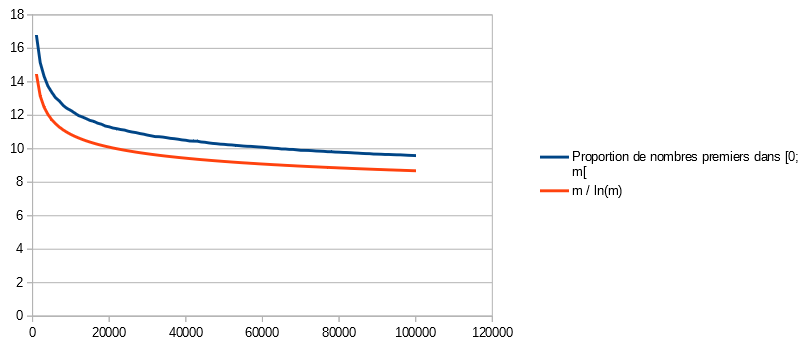
\includegraphics{prop_premier.png}
		La proportion de nombres premiers a été calculée à l'aide d'une application créée par nos soins. Elle est, sur ce graphique, exprimée en pourcentage, et les valeurs indiquées sur le graphique sont calculées à partir de m=1000 jusqu'à m=100000. Les pourcentages indiqués ici représentent donc la proportion de nombres premiers dans l'intervalle $[0; m]$.\\
		On peut constater que les courbes sont effectivement très proches, et en réalité elles le sont de plus en plus, puisque l'écart entre les deux est en moyenne décroissant. Les deux courbes tendent donc l'une vers l'autre de manière asymptotique.
		Dans l'utilisation de RSA, la partie la plus critique est la génération de nombres premiers très grands, or on sait maintenant qu'ils se raréfient au fur et à mesure que l'on cherche des nombres premiers plus grands. C'est là l'une des problématiques de RSA.